\documentclass[a4paper,10pt]{article}
\usepackage{listings}
\usepackage{graphicx}
\usepackage{color,soul}

% ----------------------------------------------------
\definecolor{hlcolor}{rgb}{1,1,0}
\sethlcolor{hlcolor}

\definecolor{light-gray}{gray}{0.90}
\lstset{language=bash}
\lstset{backgroundcolor=\color{light-gray}}

% ----------------------------------------------------
\title{Using Git to Manage CogX KTH Code}
\author{Andrzej Pronobis}


% ----------------------------------------------------
\begin{document}
\maketitle


% ----------------------------------------------------
\section{Benefits of Using Git}

\begin{itemize}
\item \textit{Branches and tags are managed by Git}. Merging can be performed easily without the need to manually track the origins of the code and worry about the same code being merged multiple times.
\item \textit{Distributed repositories}. The work can be performed locally and off-line. Branching/merging/committing does not require connection to any central server.
\item \textit{Cheap (topic) branches}. Creating local branches e.g. for testing/implementing a feature, maintenance etc. is quick and easy. A workflow based on topic branches allows to create a higher quality code and maintain stability of the master branch.
\item \textit{Commits are uniquely identified by an SHA hash code}. The SHA code is calculated based on the contents of the commit and therefore is the same even for unrelated repositories.
\item \textit{Non-linear history}. Git tracks the history of all branches and merges.
\item \textit{Performance}. Git is fast.
\end{itemize}


% ----------------------------------------------------
\section{Documentation}
\begin{itemize}
  \item Git Community Book \\
       \texttt{http://book.git-scm.com/}
  \item Git FAQ \\
       \texttt{http://git.or.cz/gitwiki/GitFaq}
  \item Git for the lazy \\
       \texttt{http://www.spheredev.org/wiki/Git\_for\_the\_lazy}
  \item Git workflow for agile teams \\
       \texttt{http://reinh.com/blog/2009/03/02/a-git-workflow-for-agile-teams.html}
  \item Git for computer scientists \\
        \texttt{http://eagain.net/articles/git-for-computer-scientists/}
\end{itemize}


% ----------------------------------------------------
\section{Installing Git}
\subsection{Ubuntu Linux}
  \begin{lstlisting}
apt-get install git-core git-gui gitk
  \end{lstlisting}

\subsection{Windows}
  Full windows installer can be found at \\
  \texttt{http://code.google.com/p/msysgit/downloads/list}



% ----------------------------------------------------
\section{Setting Up the Local Repository}
\begin{itemize}
  \item Get access to the remote repository. Generate your public SSH key:
    \begin{lstlisting}
ssh-keygen -t rsa
    \end{lstlisting}
    and send the file \texttt{$\sim$/.ssh/id\_rsa.pub} to the admin of the repository.
  \item Clone the remote repository into a local directory:
    \begin{lstlisting}
git clone git@cogvis.nada.kth.se:cogx-kth.git
    \end{lstlisting}
  \item Create local branches tracking the remote branches e.g. \texttt{year1}:
    \begin{lstlisting}
git branch --track year1 origin/year1
    \end{lstlisting}
\end{itemize}


% ----------------------------------------------------
\section{Workflow for the CogX-KTH Code}
\subsection{Overview}
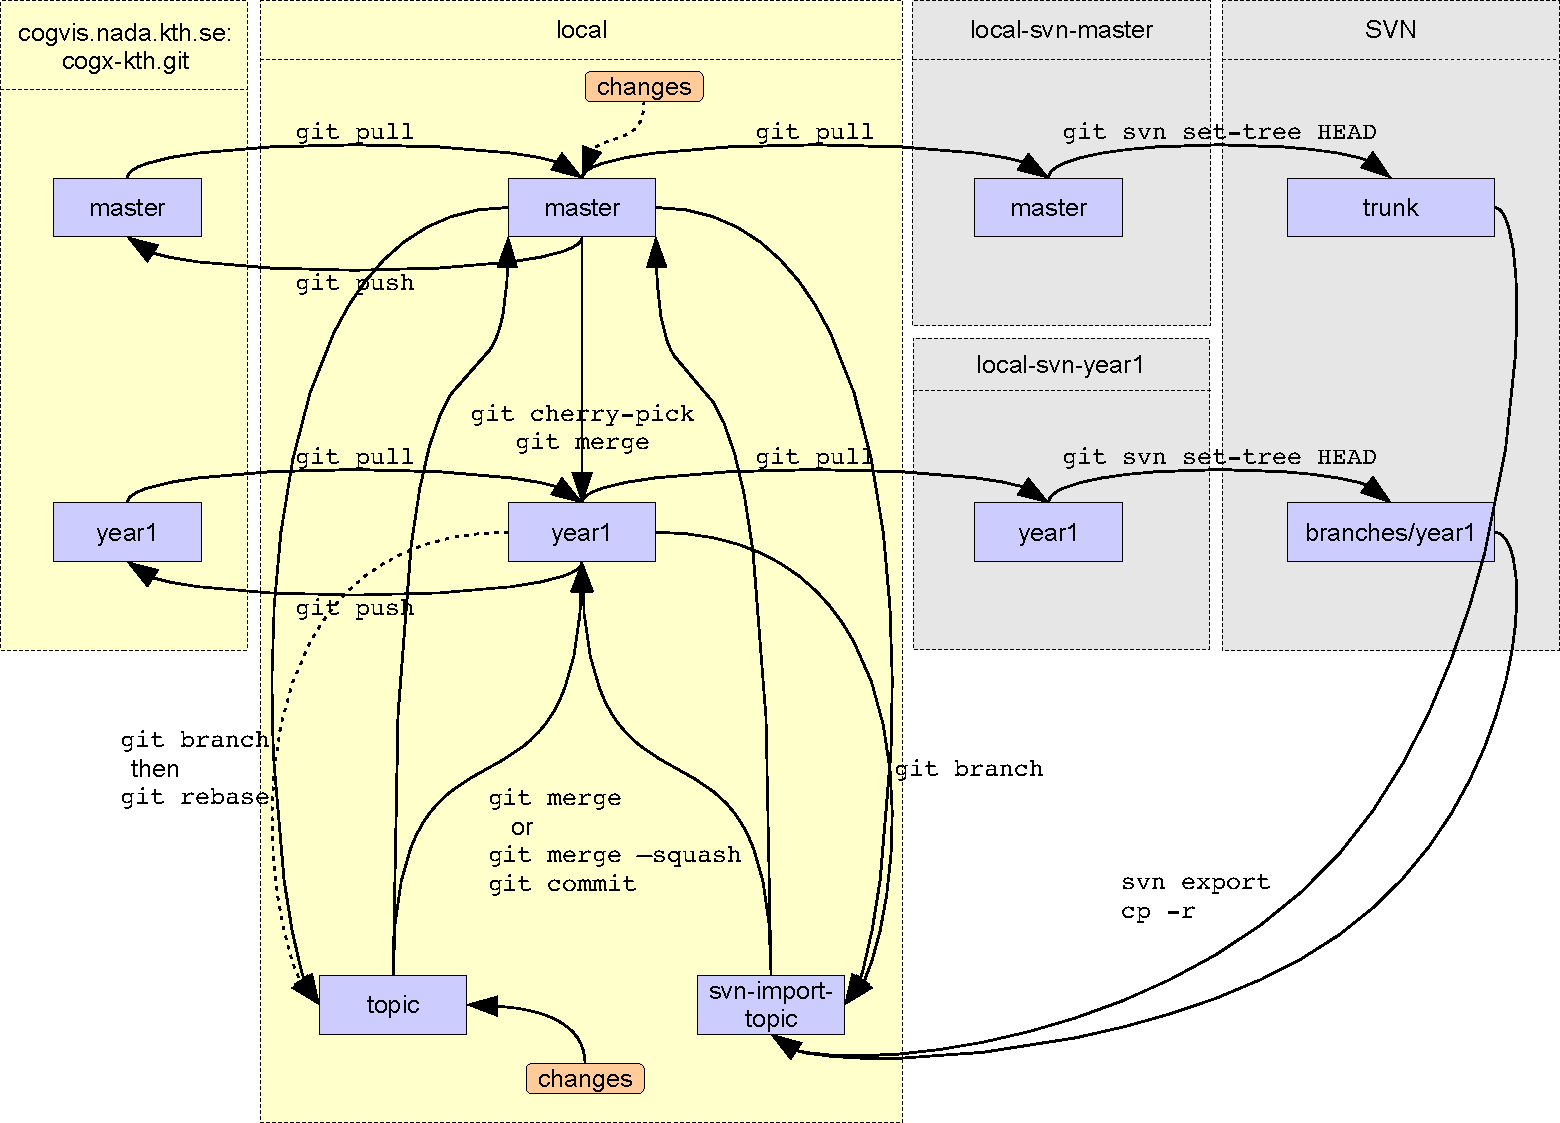
\includegraphics[width=\textwidth]{diagram}

\subsection{Feature Development}
\begin{itemize}
  \item Checkout the master branch:
    \begin{lstlisting}
git checkout master
    \end{lstlisting}
  \item Pull updates from the central server and merge them to master:
    \begin{lstlisting}
git pull
    \end{lstlisting}
  \item Create and checkout a topic branch for the new feature:
    \begin{lstlisting}
git checkout -b topic
    \end{lstlisting}
  \item Do some work in the topic branch:
    \begin{lstlisting}
echo "contents" > file
git add file
git commit -m "First commit"
echo "contents2" > file2
git add file2
git commit -m "Second commit"
    \end{lstlisting}
  \item Merge with the master branch:
    \begin{lstlisting}
git checkout master
git merge --squash topic
git commit
    \end{lstlisting}
  \item Push the changes upstream:
    \begin{lstlisting}
git push
    \end{lstlisting}
  \item Do more work in the topic branch:
    \begin{lstlisting}
git checkout topic
echo "new contents" > file
git add file
git commit -m "Third commit"
    \end{lstlisting}
  \item Pull some new updates from the central server and merge them to master:
    \begin{lstlisting}
git checkout master
git pull
    \end{lstlisting}
  \item Rebase the topic branch against the new changes:
    \begin{lstlisting}
git checkout topic
git rebase master
    \end{lstlisting}
  \item Merge the changes with the master branch:
    \begin{lstlisting}
git checkout master
git merge --squash topic
git commit
    \end{lstlisting}
  \item Push the changes upstream:
    \begin{lstlisting}
git push
    \end{lstlisting}



\subsection{Pushing Changes to SVN}
\hl{Missing}


\subsection{Pulling Changes from SVN}
\hl{Missing}




\end{itemize}



% ----------------------------------------------------
\section{FAQ}
\begin{enumerate}
  \item How to list branches and check which branch is checked out?
    \begin{lstlisting}
git branch
    \end{lstlisting}
  \item How to list all branches including remote branches?
    \begin{lstlisting}
git branch -a
    \end{lstlisting}
  \item How to view history of a branch or all branches?
    \begin{lstlisting}
gitk
gitk --all
    \end{lstlisting}
  \item How to throw away uncommitted change in a single file?
    \begin{lstlisting}
git checkout -- file
    \end{lstlisting}

\end{enumerate}


\end{document}
